\iffalse
\subsection{Lifetime Contributions of Reciprocity-Activated Users}
%\placeholder{Include comparison of lifetime contributions for users whose first help was within seven days of receiving an answer vs.\ users whose first help was outside this window.}

\subsection{Alternative Observation Windows}
\label{sec:robustness_windows}
%\placeholder{Include results with 3-day, 5-day, and 14-day observation windows showing qualitative robustness of main findings.}

\subsection{Restricted Experience Analysis}
\label{sec:robustness_restricted}
%\placeholder{Include analysis restricted to users' first six activities, showing that reciprocity decline and response time moderation hold even within a narrow experience range.}

\subsection{Falsification Test}
\label{sec:falsification}
%\placeholder{Include results of the gap-period falsification test showing no significant effect during the waiting period.}

\subsection{Full Regression Tables}
\label{sec:full_tables}
%\placeholder{Include complete regression output for all models across all tenure buckets, including all covariates, standard errors, and model diagnostics.}
\fi

\section{Replication materials}
Analysis code and instructions to reproduce all tables and figures are available in a public repository (URL withheld for blind review).

\section{Matching Diagnostics}
\label{sec:balance_plot}
Figure \ref{fig:common_support} shows that there is sufficient common support between the treatment and the control group. The propensity score distribution between the original treated and control groups is similar. The distribution of the matched control is nearly identical to the treated group. 

\begin{figure}[!htbp]
    \centering
    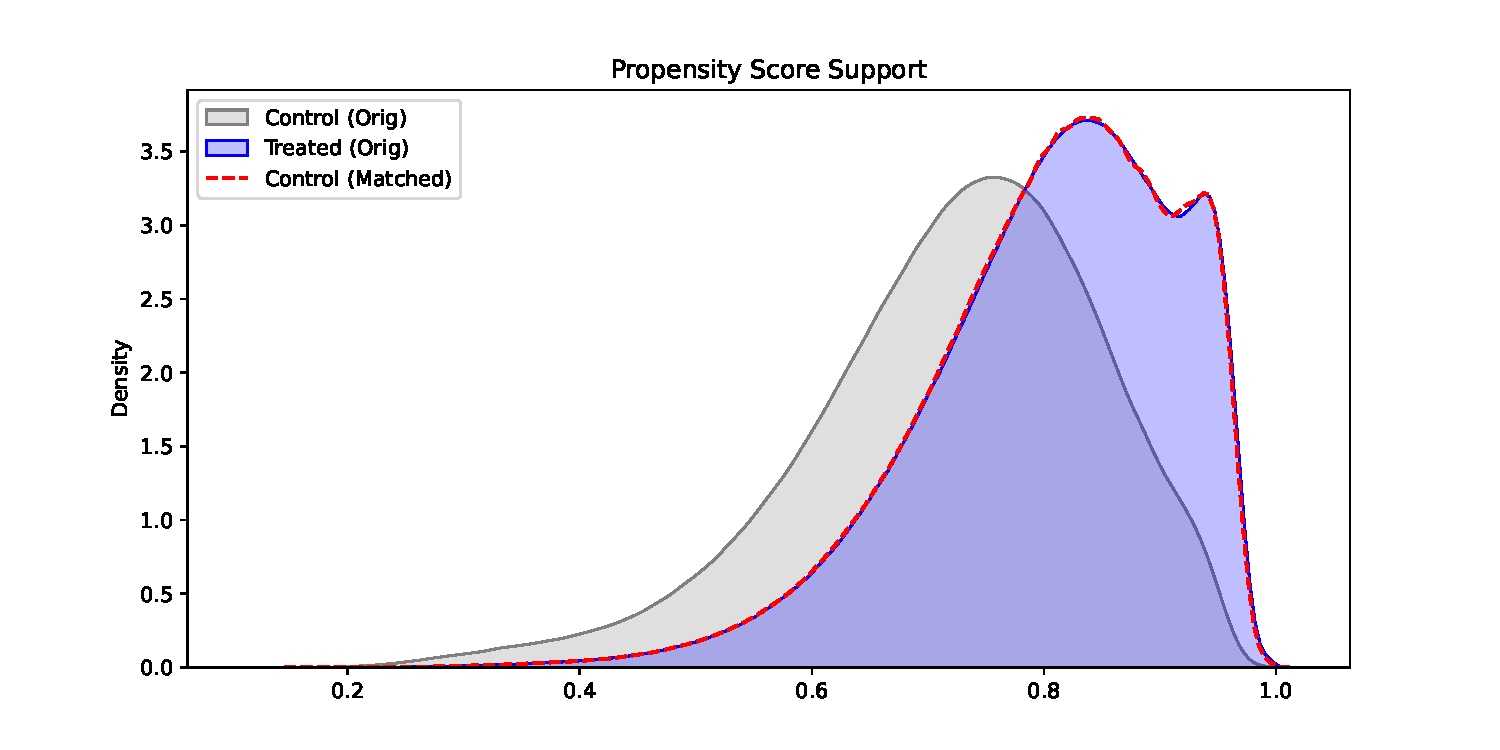
\includegraphics[width=\textwidth]{matching/common_support.pdf}
    \caption{Distribution of propensity scores of treatment group, control group, and matched control group}
    \label{fig:common_support}
\end{figure}

Figure \ref{fig:love_plot} displays the standardized mean differences (SMD) between the matching variables before and after matching. While there are noticeable differences before the matching, all SMDs are very close to zero after the matching. 

\begin{figure}[!htbp]
    \centering
    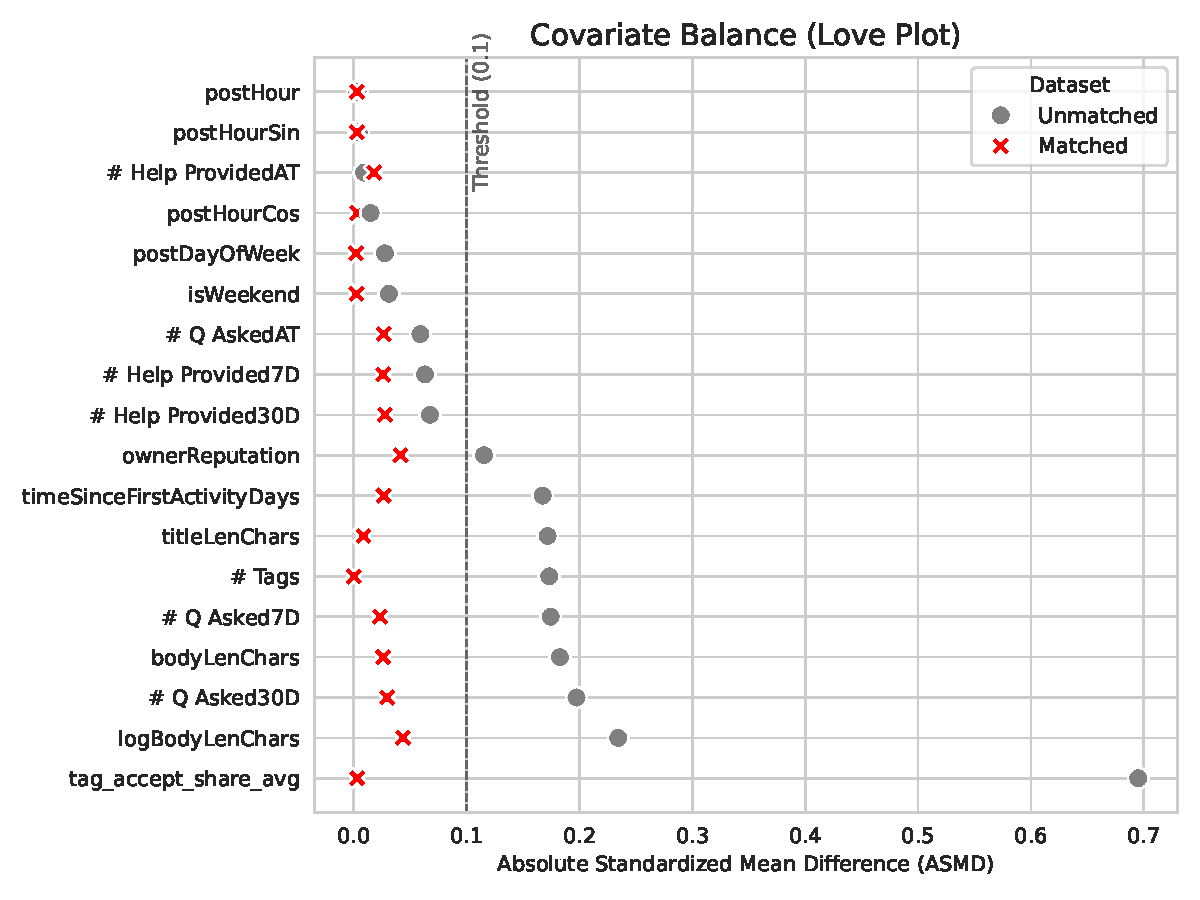
\includegraphics[width=\textwidth]{matching/love_plot.pdf}
    \caption{Visualization of balance in the unmatched and matched dataset}
    \label{fig:love_plot}
\end{figure}

\section{Help Rate Over the Observation Window by Tenure}
\label{sec:help_rate_by_tenure}

\begin{figure}[!htbp]
\centering
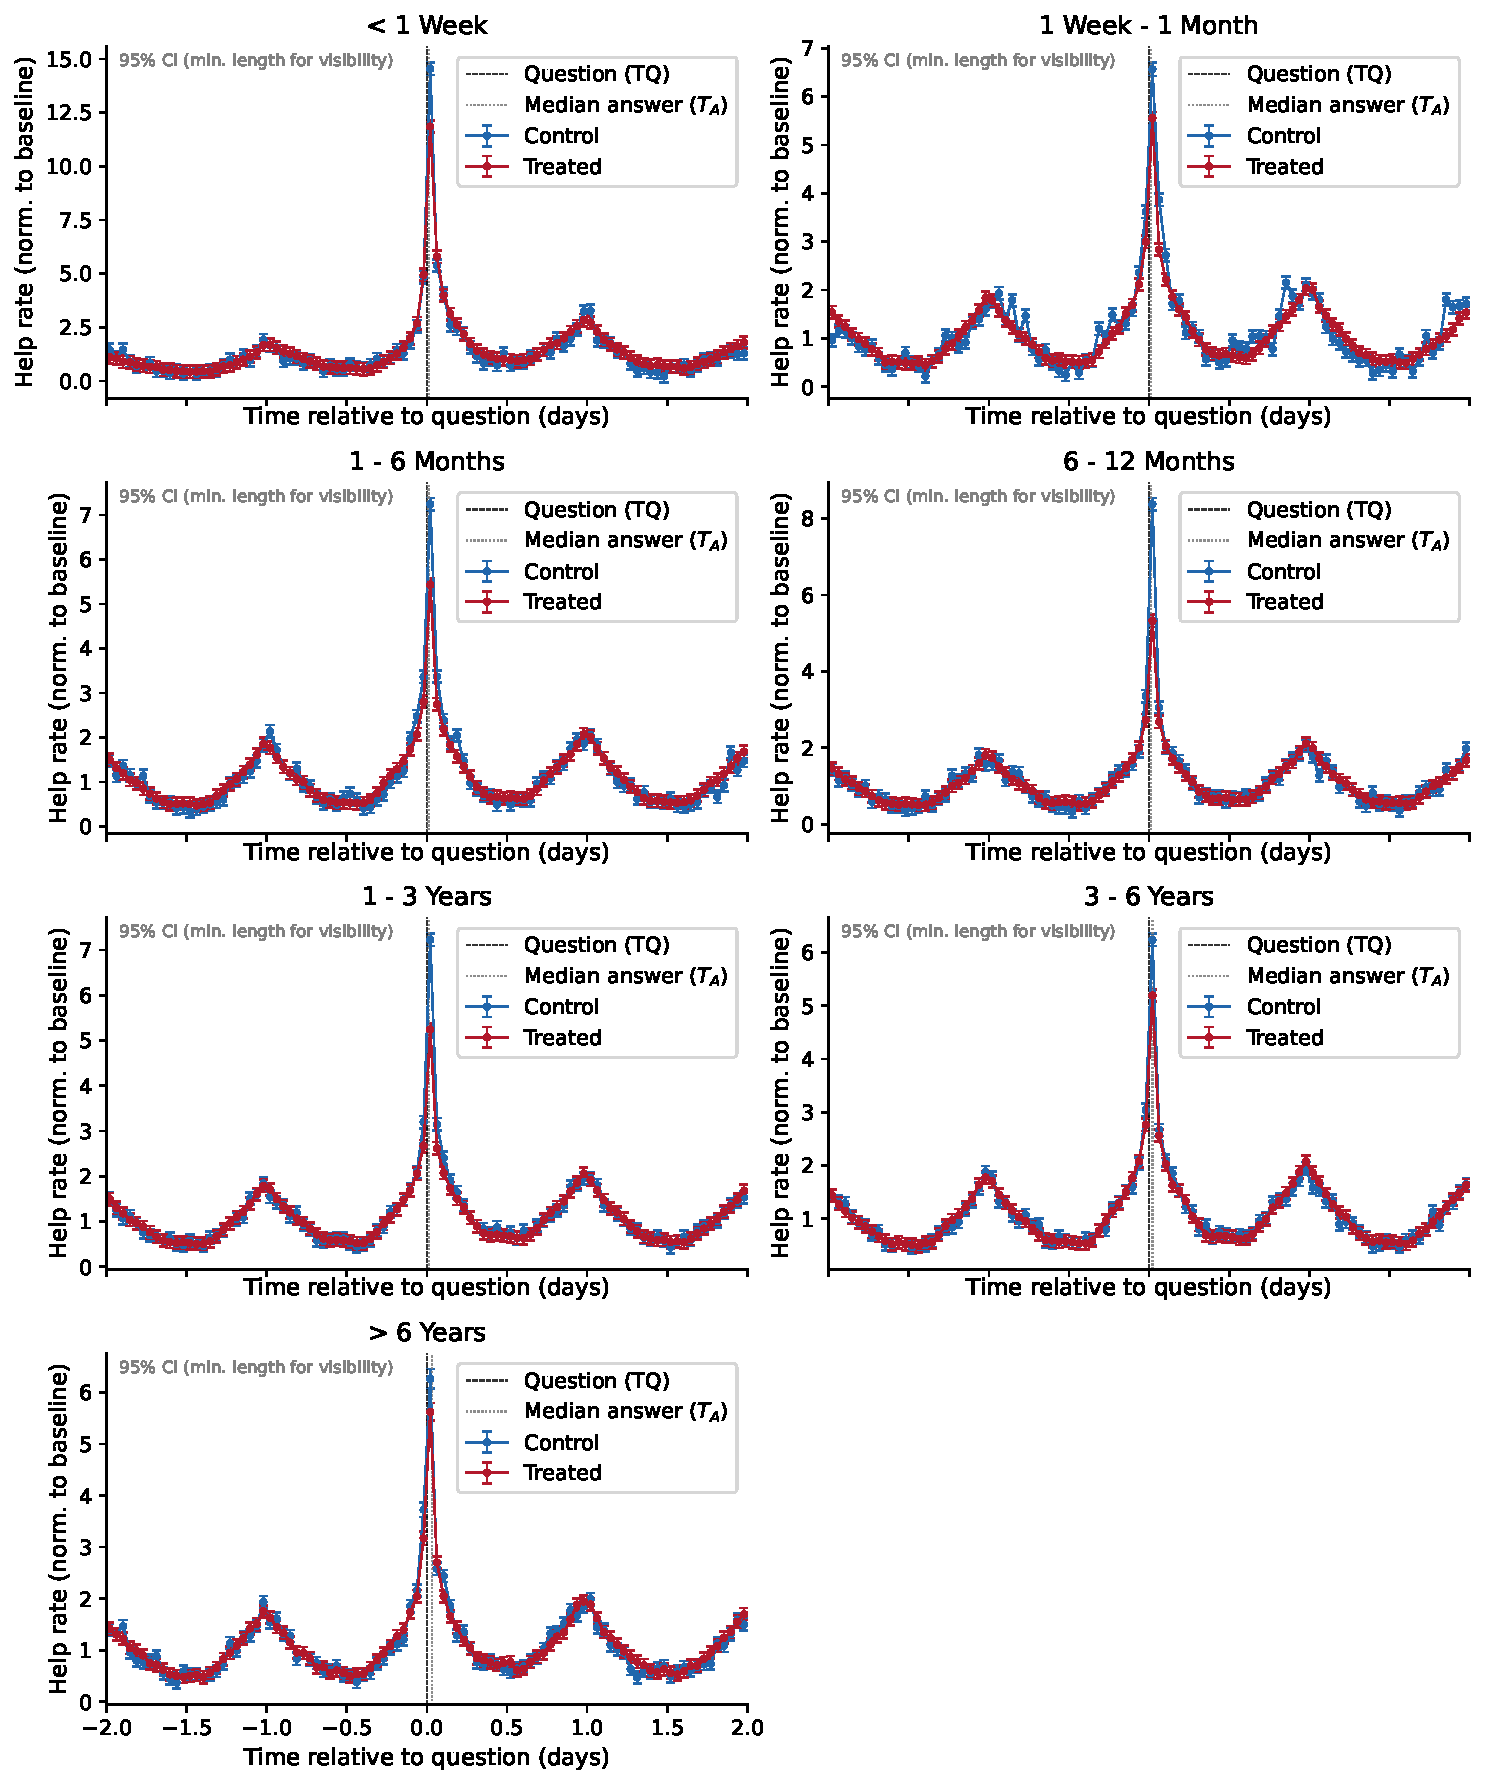
\includegraphics[width=\textwidth]{analysis/output_figures/help_rate_by_tenure.pdf}
\caption{Help Rate Over the Observation Window, by Tenure Bucket. Each panel plots the normalized help rate (relative to each group's pre-question baseline) for treated users (red) and matched control users (blue) over the $\pm$2-day window around the question-posting time ($T_Q$, dashed vertical line). The dotted vertical line marks the median answer arrival time ($T_A$). Error bars indicate 95\% confidence intervals.}
\label{fig:help_rate_by_tenure}
\end{figure}

Figure \ref{fig:help_rate_by_tenure} shows that the post-question lift in treated users' help rate is visible across all tenure buckets and is most pronounced among newcomers (tenure $<$ 1 week), consistent with the pattern reported in Table~\ref{tab:main_results} and Figure~\ref{fig:strength_rec}.

\section{Help Rate by Adoption Status and Tenure Bucket}
\label{sec:help_rate_adoption_by_tenure}

\begin{figure}[!htbp]
\centering
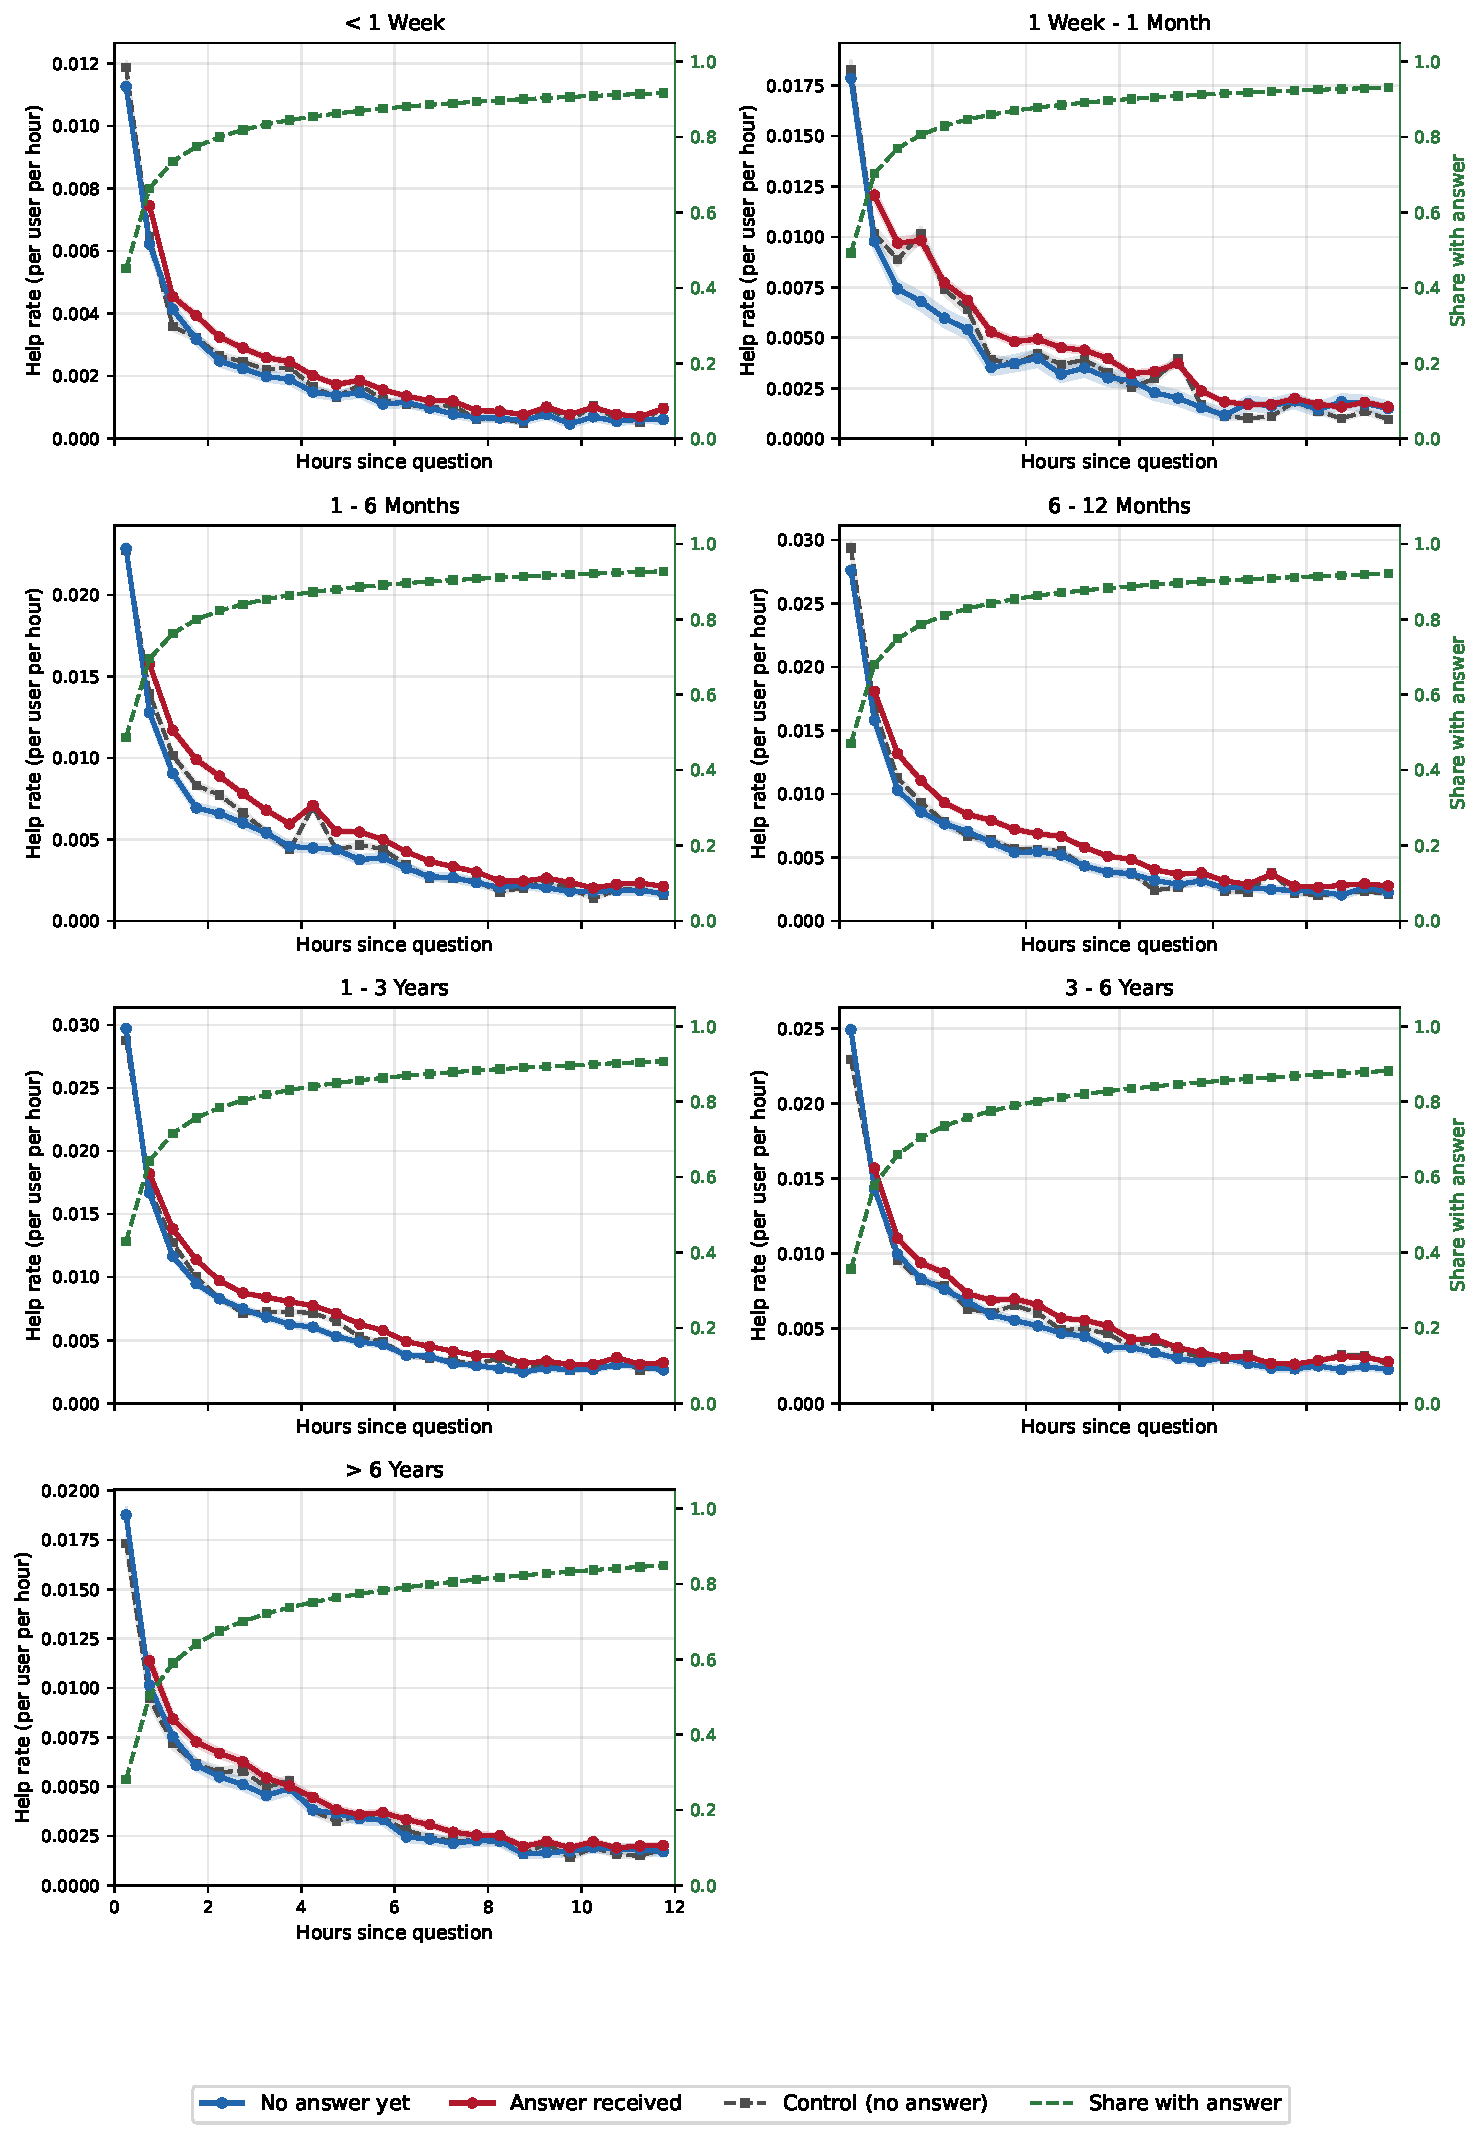
\includegraphics[width=.9\textwidth]{analysis/output_figures/help_rate_adoption_by_tenure.pdf}
\caption{Help rate in the post-question window by answer-receipt status, separately by tenure bucket. %Dark blue dashed: matched control users who received no answer. Blue: treated users who have not yet received an answer (``No answer yet''). Red: treated users who have already received an answer (``Answer received''). Green dashed (right axis): cumulative share of treated users who have received an answer by each hour.
}
\label{fig:help_rate_adoption_by_tenure}
\end{figure}

Figure \ref{fig:help_rate_adoption_by_tenure} shows that for experienced users (all panels beyond $<$\,1 Week), the help rate of users still waiting (blue) exceeds that of users who have already received an answer (red), and both exceed the control baseline (grey dashed), up to approximately 1--2 hours post-question. This is consistent with the re-engagement window account: the pending-question state elevates engagement, and answer receipt collapses it back toward control levels. The newcomer panel ($<$\,1 Week) shows the reverse ordering, consistent with the gratitude-and-obligation mechanism dominating for users who do not promptly exit after receiving help.

\section{Selection Sensitivity and Absolute Effects}
\label{sec:selection_absolute}

Table~\ref{tab:selection_bounds} reports transparent bounds on the reciprocity contrast under alternative assumptions about zero-event controls. Table~\ref{tab:absolute_effects} translates the tenure-bucket hazard ratios into absolute-risk-difference proxies using observed baseline event rates.

\begin{table}[H]
\caption{Selection Sensitivity Based on Zero Post-Question Helping}
\label{tab:selection_bounds}
\centering
\footnotesize
\begin{tabular}{@{}lrrrr@{}}
\toprule
\textbf{Scope} & \textbf{Assumed frac.} & \textbf{Base HR} & \textbf{Control zero share} & \textbf{Adjusted RR proxy} \\
\midrule
All & 0.00 & 0.29 & 89.9% & 3.85 \\
All & 0.10 & 0.29 & 89.9% & 2.70 \\
All & 0.25 & 0.29 & 89.9% & 1.86 \\
All & 0.50 & 0.29 & 89.9% & 1.23 \\
$<$ 1 Week & 0.00 & 0.26 & 90.1% & 2.98 \\
$<$ 1 Week & 0.10 & 0.26 & 90.1% & 2.01 \\
$<$ 1 Week & 0.25 & 0.26 & 90.1% & 1.36 \\
$<$ 1 Week & 0.50 & 0.26 & 90.1% & 0.88 \\
1 Week - 1 Month & 0.00 & 0.28 & 88.8% & 3.46 \\
1 Week - 1 Month & 0.10 & 0.28 & 88.8% & 2.47 \\
1 Week - 1 Month & 0.25 & 0.28 & 88.8% & 1.73 \\
1 Week - 1 Month & 0.50 & 0.28 & 88.8% & 1.15 \\
1 - 6 Months & 0.00 & 0.29 & 88.4% & 3.54 \\
1 - 6 Months & 0.10 & 0.29 & 88.4% & 2.59 \\
1 - 6 Months & 0.25 & 0.29 & 88.4% & 1.84 \\
1 - 6 Months & 0.50 & 0.29 & 88.4% & 1.24 \\
6 - 12 Months & 0.00 & 0.30 & 88.5% & 3.76 \\
6 - 12 Months & 0.10 & 0.30 & 88.5% & 2.74 \\
6 - 12 Months & 0.25 & 0.30 & 88.5% & 1.96 \\
6 - 12 Months & 0.50 & 0.30 & 88.5% & 1.32 \\
1 - 3 Years & 0.00 & 0.30 & 89.6% & 4.05 \\
1 - 3 Years & 0.10 & 0.30 & 89.6% & 2.89 \\
1 - 3 Years & 0.25 & 0.30 & 89.6% & 2.02 \\
1 - 3 Years & 0.50 & 0.30 & 89.6% & 1.34 \\
3 - 6 Years & 0.00 & 0.29 & 91.6% & 4.53 \\
3 - 6 Years & 0.10 & 0.29 & 91.6% & 3.02 \\
3 - 6 Years & 0.25 & 0.29 & 91.6% & 2.01 \\
3 - 6 Years & 0.50 & 0.29 & 91.6% & 1.29 \\
$>$ 6 Years & 0.00 & 0.29 & 93.5% & 5.74 \\
$>$ 6 Years & 0.10 & 0.29 & 93.5% & 3.37 \\
$>$ 6 Years & 0.25 & 0.29 & 93.5% & 2.08 \\
$>$ 6 Years & 0.50 & 0.29 & 93.5% & 1.27 \\
\bottomrule
\multicolumn{5}{@{}l}{\footnotesize Assumed frac. is the fraction of zero-post-help control questions assigned one latent help event.} \\
\multicolumn{5}{@{}l}{\footnotesize Adjusted RR is an event-rate proxy, not a refitted Cox hazard ratio.} \\
\end{tabular}
\end{table}

\begin{table}[H]
\caption{Absolute Effect Sizes and NNT}
\label{tab:absolute_effects}
\centering
\footnotesize
\begin{tabular}{@{}lrrrrrr@{}}
\toprule
\textbf{Row} & \textbf{Base risk} & \textbf{HR} & \textbf{ARD} & \textbf{NNT} & \textbf{NNT CI} & \textbf{Summed HR} \\
\midrule
$<$ 1 Week & 0.1181 & 1.059 & 0.00697 & 143.5 & 112.6--196.9 & 1.107 \\
1 Week - 1 Month & 0.2001 & 1.021 & 0.00417 & 240.1 & 121.9--4868.1 & 0.988 \\
1 - 6 Months & 0.2341 & 1.043 & 0.01001 & 99.9 & 75.3--147.5 & 1.022 \\
6 - 12 Months & 0.2548 & 1.042 & 0.01073 & 93.2 & 70.4--136.9 & 1.026 \\
1 - 3 Years & 0.2446 & 1.027 & 0.00664 & 150.5 & 101.7--286.5 & 1.028 \\
3 - 6 Years & 0.1986 & 1.008 & 0.00155 & 645.2 & — & 1.003 \\
$>$ 6 Years & 0.1428 & 0.981 & -0.00271 & — & — & 0.993 \\
AllData\_Main & 0.2064 & 1.002 & 0.00050 & 1995.0 & — & 1.008 \\
\bottomrule
\multicolumn{7}{@{}l}{\footnotesize HR/ARD/NNT are the primary (headline) estimand; ``Summed HR'' is the summed DiD ($\exp(\beta_2+\beta_4)$, upper bound).} \\
\end{tabular}
\end{table}

\section{Analysis of Life-Time Contributions}
\label{sec:lt-contributions}
What remains unclear is whether users who become contributors through generalized reciprocity continue to contribute consistently and become valuable community members. To explore this, we compare the contributions of reciprocity-activated users with those of all contributors selected for Study 1. Specifically, we examine the number of times users from each group provided and received help up to July 14, 2024. The results are presented in Table \ref{tab:quartile_statistics}. Across all quartiles and at the median, reciprocity-activated users ask and provide more help than their counterparts.
For example, at the median, reciprocity-activated users provide eight answers and ask 13 questions, compared to six answers and 11 questions among all contributors. Similarly, the 75th percentile of reciprocity-activated users provides 23 answers and asks 29 questions, compared to 19 answers and 22 questions for all contributors.
These findings suggest that users who begin contributing after receiving help become equally, if not more, engaged in the community's helping dynamics compared to all contributors. Furthermore, this analysis demonstrates that once users start contributing, the act of giving and receiving help becomes (at least temporarily) decoupled.

\begin{table}[H]
\caption{Statistics on Contributions by User Sample}
\label{tab:quartile_statistics}
\centering
\begin{tabular}{lcccccc}
\toprule
 & \multicolumn{3}{c}{Answers Provided} & \multicolumn{3}{c}{Questions Asked} \\
\cmidrule(lr){2-4} \cmidrule(lr){5-7}
 & $Q_1$ & Med & $Q_3$ & $Q_1$ & Med & $Q_3$ \\
\midrule
Reciprocity-activated (\(N = 30,160\)) & 3.0 & 8.0 & 23.0 & 7.0 & 13.0 & 29.0 \\
All Contributors (\(N = 287,959\)) & 2.0 & 6.0 & 19.0 & 6.0 & 11.0 & 22.0 \\
\bottomrule
\end{tabular}
\end{table}

\iffalse
\begin{table}[caption={Linear Regression Results on Lifetime Contributions}, label={tab:quartile_statistics}]
\centering
\begin{tabular}{@{\extracolsep{1pt}}lcc} \toprule
& \multicolumn{2}{c}{Dependent Variable} \\ \cmidrule(lr){2-3}
& logNumberAnswers & logNumberComments \\
\midrule
activatedUser(1) & 0.081$^{***}$ & 0.187$^{***}$ \\ 
 & (0.007) & (0.010) \\ \rule{0pt}{4ex}%
 
numberQuestions & 0.007$^{***}$ & 0.008$^{***}$ \\ 
 & (0.000) & (0.001) \\ \rule{0pt}{4ex}%

Constant & 3.413$^{***}$ & 2.925$^{***}$ \\
 & (0.016) & (0.023) \\ \rule{0pt}{4ex}%
Year controls & YES & YES \\
\midrule
Observations & 287,959 & 287,959 \\
F-statistic & 3168$^{***}$ & 2498$^{***}$ \\ 
\bottomrule
\end{tabular}
\caption*{\raggedright \textit{Notes.} Significance levels: $^{*}$ \textit{p} < .05; $^{**}$\textit{p} < .01; $^{***}$\textit{p} < .001. Standard errors are reported in parentheses.}
\end{table}
\fi

\iffalse
\section{Robustness Checks \label{sec:robustness}}
To assess the robustness and consistency of my findings, I conducted a series of robustness checks that varied the observation length, the construction of the dependent variable \textit{numHelped}, or model specification.

I assessed the robustness of my findings by varying the observation length. While the reciprocity model used a seven-day observation length per period, I created two equivalent models with ten and three days of observation length. That is, I observe the helping behavior of the user three and ten days before and after receiving help, respectively. The results of these additional models (see Table \ref{tab:rec_models10d} and \ref{tab:rec_models3d}) are consistent with the above results and qualitatively equivalent, indicating that the findings are not sensitive to the specific observation length used.
\fi


\section{Implementation Details} All models are estimated using the \texttt{lifelines} CoxTimeVaryingFitter with a small ridge (L2) penalizer applied for numerical stability. The penalizer strength is $\lambda = 5 \times 10^{-3}$ for main-effect models and $\lambda = 10^{-2}$ for models that include response-time interaction terms (where the interaction covariates are correlated with the base treatment indicator). These values are sufficiently small that they introduce negligible shrinkage relative to the scale of the estimated effects, but they ensure stable Hessian inversion in large risk sets. All covariates are mean-centered before fitting; response-time interaction terms are additionally clipped to their 5th--95th percentile range and z-scored as described above. Table standard errors are model-based; matched-pair bootstrap uncertainty is reported separately when generated. Because matched pairs are constructed across different users and the time-varying covariate structure eliminates the need for within-user corrections, this approach is appropriate; we note that clustering at the match level would be the natural extension if robust SEs were desired. For the pooled experienced-user models (H1), estimation was performed on a random sample of approximately 8,001,931 user-interval rows drawn from matched pairs (preserving pair integrity) to keep computation feasible; tenure-bucket-specific models (H2, H3) use all available intervals within each stratum.